\subsection{Фазовые траектории одномерной модели.}

Поверхность вращательной энергии является мощным инструментом, позволяющим на качественном уровне анализировать вращательную динамику молекулярной системы. Однако с ростом полной колебательно-вращательной энергии влияние колебательной подсистемы на вращение молекулы не может быть точно учтено в рамках эффективного гамильтониана. Следовательно необходимо решать полную систему динамических уравнений. При решении полной системы динамических уравнений необходимо надлежащим образом задавать начальные условия. \\

Система динамических уравнений, полученная из гамильтониана \eqref{model_ham}, выглядит следующим образом:
\vverh
\begin{gather}
\left\{
\begin{aligned}
\dot{\Phi} &= \left( \frac{J \cos \Phi \sin \Theta}{I_0 ( 1 - \cos q)} \cos \Phi + \frac{J \sin \Phi \sin \Theta}{2I_0} \sin \Phi \right) \ctg \Theta - \frac{J \cos \Theta}{I_0 (1 + \cos q)} \\
\dot{\Theta} &= \frac{J \cos \Phi \sin \Theta}{I_0 (1 - \cos q)} \sin \Phi - \frac{J \sin \Phi \sin \Theta}{2I_0} \cos \Phi \\
\dot{q} &= 2	\frac{p}{I_0} \\
\dot{p} &= - \frac{\sin q}{2I_0} \left( \frac{J^2 \cos^2 \Theta}{(1 + \cos q)^2} - \frac{J \cos^2 \Phi \sin^2 \Theta}{(1 - \cos q)^2} \right) - \frac{1}{2I_0} \left( \frac{V_{+} \sin q}{(1 + \cos q)^2} - \frac{V_{-} \sin q}{(1 - \cos q)^2} \right)
\end{aligned}
\right. \notag
\end{gather}

Решение представленной системы дифференциальных уравнений производилось при помощи математической платформы \textit{Maple 2015}. Возвращаясь к вопросу начальных условий, в качестве начального значения деформационного угла удобно использовать $q_0 = q_e$ (равновесного значения $q$ при фиксированном значении модуля вектора углового момента $J$). Переписывая выражение модельного гамильтониана \eqref{model_ham} через эффективный потенциал $V_{eff.}$, несложно получить начальное значение имупльса:
\vverh
\begin{gather}
E_n = \frac{p_0^2}{I_0} + V_{eff.} (q_0) \quad \implies \quad p_0 = \sqrt{I_0 \cdot \left( E_n - V_{eff.} (q_0) \right) } \notag
\end{gather}

Отметим, что положение $E_n$ внутри энергетической полосы (рисунок \eqref{vib_levels}) с номером $n$ определяется углами $\Theta_0$, $\Phi_0$, характеризующими направление вектора углового момента. Подводя итог вышесказанному, проиллюстрируем определение начальных условий системы динамических уравнений в виде блок-схемы.

\vverh
\begin{figure}[H]
  \begin{center}
    \begin{tikzpicture}[framed]
      \tikzstyle{type1} = [rectangle, rounded corners, minimum width = 3cm, minimum height = 1cm, text centered, text width = 3cm ,draw = black, fill = yellow!30]

\tikzstyle{type2} = [rectangle, rounded corners, minimum width = 3cm, minimum height = 1cm, text centered, text width = 3cm, draw = black, fill = green!30]

\tikzstyle{arrow} = [thick, ->, >=stealth]

\node (angles) [type1] {$\Theta_0, \Phi_0$};

\node (moments) [type2, below = 1.5 cm of angles] {$J_{x,0}, J_{y, 0}, J_{z, 0}$};

\node (energy) [type2, right = 1.5 cm of moments] {$E_n$};

\node (excitation_level) [type1, right = 1.5cm of angles] {$n$};

\node (effective_potential) [type2, right = 1.5 cm of excitation_level] {$V_{eff.} = V_{eff.}(q_e)$};

\node (q_angle) [type1, right = 1.5 cm of effective_potential] {$q = q_e$};

\node (p) [type1, below = 1.5 cm of effective_potential] {$p_0$};

\draw [arrow] (angles) -- (moments);
\draw [arrow] (moments) -- (energy);
\draw [arrow] (energy) -- (p);
\draw [arrow] (excitation_level) -- (energy);
\draw [arrow] (q_angle) -- (effective_potential);
\draw [arrow] (effective_potential) -- (p); 
	  \begin{scope}[on background layer]
      \node [fill=black!30,fit= (angles) (moments) (energy) (excitation_level) (q_angle) (p)] {};
      \end{scope}
    \end{tikzpicture}
    \caption{Схема определения начальных параметров системы.}
  \end{center}
\end{figure}

В результате решения системы дифференциальных уравнений мы получаем функции сферических углов $\Theta(t)$, $\Phi(t)$, функции обобщенных координат $q(t)$ и импульса $p(t)$, зависящие от времени. Фазовым пространством вращательной подзадачи является двумерная сфера, радиус которой равен модулю вектора углового момента (который является интегралом движением). Фазовые траектории, лежащие на двумерной сфере, описывают динамику конца вектора углового момента и задаются парой углов $\Phi, \Theta$, которые мы и получаем в результате решения полной системы динамических уравнений. Таким образом, мы имеем возможность проанилизировать изменения, происходящие с фазовым портретом вращательной подзадачи. На рисунке \eqref{fig:rigid_base1} представлена серия фазовых траекторий основного колебательного состояния ($n = 0$), начинающихся в одной точке фазового пространства  -- $\Phi_0 = 0 \, \text{рад.}$, $\Theta_0 = 0.15 \, \text{рад.}$ , но при разных значениях модуля вектора углового момента $J$. Для удобства траектории представлены на сферах одинакового радиуса.

\begin{figure}[H]
  \centering
	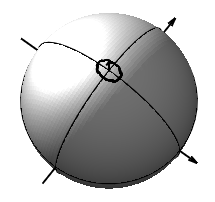
\includegraphics[width=0.3\textwidth]{../pictures/rigid_base/plot_J=10n=0.png}
	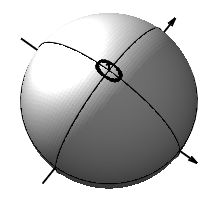
\includegraphics[width=0.3\textwidth]{../pictures/rigid_base/plot_J=15n=0.png}
	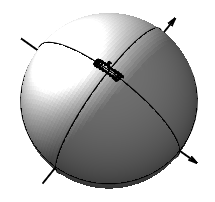
\includegraphics[width=0.3\textwidth]{../pictures/rigid_base/plot_J=20n=0.png} \\
	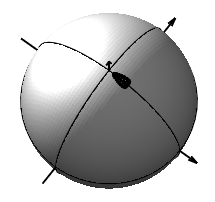
\includegraphics[width=0.3\textwidth]{../pictures/rigid_base/plot_J=21n=0.png}
	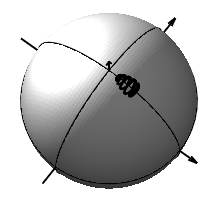
\includegraphics[width=0.3\textwidth]{../pictures/rigid_base/plot_J=22n=0.png} \\
	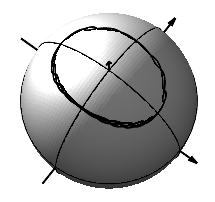
\includegraphics[width=0.3\textwidth]{../pictures/rigid_base/plot_J=10n=0theta=75.png}
	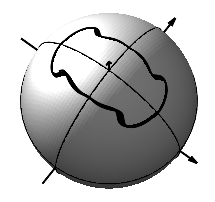
\includegraphics[width=0.3\textwidth]{../pictures/rigid_base/plot_J=21n=0theta=75.png}
	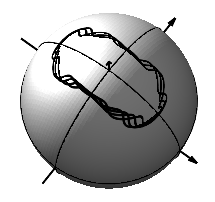
\includegraphics[width=0.3\textwidth]{../pictures/rigid_base/plot_J=22n=0theta=75.png}
	\caption{Динамика вектора углового момента модельной системы с деформационной степенью свободы в основном колебательном состоянии. Начальные параметры системы: \
	\textbf{первый ряд} : $\Phi_0 = 0$, $\Theta_0 = 0.15$, $J = 10, \, 15, \, 20$ (\textit{до бифуркации});
	\textbf{второй ряд} : $\Phi_0 = 0$, $\Theta_0 = 0.15$, $J = 21, \, 22$ (\textit{после бифуркации});
	\textbf{третий ряд} : $\Phi_0 = 0$, $\Theta_0 = 0.75$, $J = 10$ (\textit{до бифуркации}), $21, \, 22$ (\textit{после бифуркации}).}
	\label{fig:rigid_base1}
\end{figure}

Поведение фазовых траекторий в основном колебательном состоянии несколько отличается от траекторий в других колебательных состояниях. При значениях углового момента меньших критического $J < J_{cr.}$ фазовые траектории описывают замкнутые контуры вокруг оси $Oz$, которые с ростом $J$ уплощаются, прижимаясь к оси $Oy$. При достижении критического значения $J = J_{cr.}$ фазовая траектория ''перескакивает'', начинает концентирироваться вокруг новой оси устойчивого вращения. Новые фазовые траектории качественно отличаются от предыдущих -- они начинают плотным образом заметать область, а не описывать контуры вокруг оси. По виду фазовых траекторий мы можем определить примерное значение критического значения момента -- $J_{cr.} \approx 21-22$. Появление траекторий такого типа подтверждает наличие четырехкратно-вырожденных кластеров в верхней части вращательного мультиплета.

\begin{figure}[H]
  \centering
	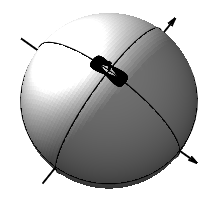
\includegraphics[width=0.3\textwidth]{../pictures/rigid_base/plot_J=20n=1.png}
	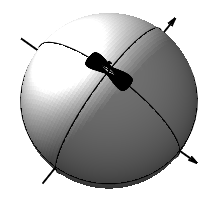
\includegraphics[width=0.3\textwidth]{../pictures/rigid_base/plot_J=21n=1.png}
	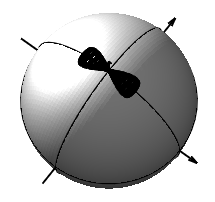
\includegraphics[width=0.3\textwidth]{../pictures/rigid_base/plot_J=22n=1.png} \\
	\caption{Динамика вектора углового момента модельной системы с деформационной степенью свободы в первом колебательном состоянии. Начальные параметры системы: \ $\Phi_0 = 0$, $\Theta_0 = 0.15$, $J = 20, \, 21, \, 22$.}
	\label{fig:rigid_base2}
\end{figure}

В первом колебательном состоянии наблюдается фазовая траектория, которая доказывает смену характера устойчивости оси вращения, распологающейся вдоль оси $Oz$. Траектории, показанные на рисунке \eqref{fig:rigid_base2}, изображают восьмерку и локализуется вокруг новых устойчивых осей вращения, что указывает на существование особой точки типа "центр" в центре восьмерки. \\
С ростом колебательного возбуждения наблюдается уменьшение критического значения $J_{cr.}$. Помимо этого, происходит постепенная делокализация траекторий, что приводит к исчезновению четырехкратно-вырожденных кластеров из вращательного спектра.